\chapter{ADM-Archimate}
\section{Introducción}
contenido...
\newpage

\section{ADM}
contenido...

\begin{figure}[h!]
	\centering
	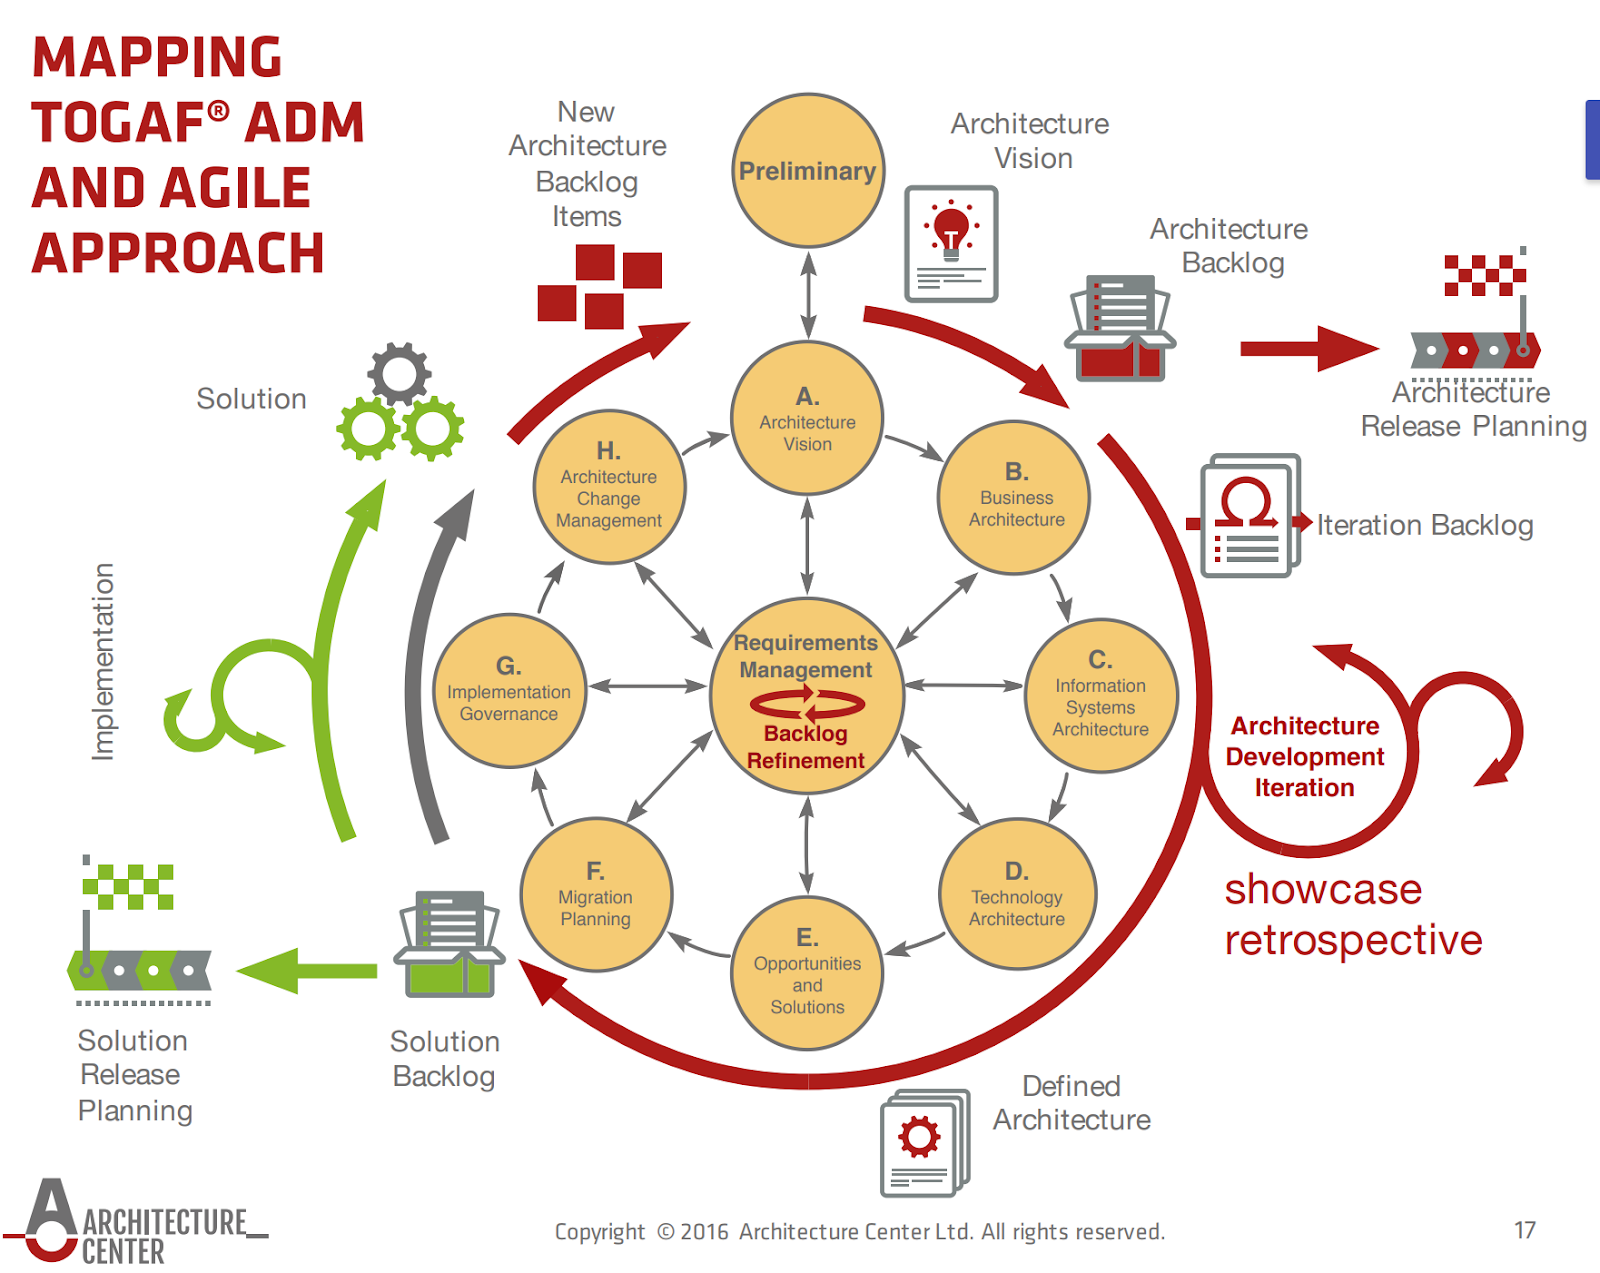
\includegraphics[width=0.7\linewidth]{ARQUITECTURA/imgs/adm}
	\caption{ADM \cite{SB,1579133,6337726,6337730,6827125}}
\end{figure}


\newpage

\section{Archimate}
contenido...

\newpage

\section{Caso de Estudio}
contenido...

\subsection{Misión}
Ofrecer a nuestros clientes el mejor servicio de desarrollo de herramientas tecnologías con contenido novedoso y útil. Para ello implementamos soluciones creativas adaptadas a las necesidades del cliente.
\subsection{Visión}
En el 2025 queremos ser una empresa líder en la creación de desarrollo de herramientas tecnologías móviles a nivel nacional, ofreciendo soluciones prácticas, empleado conocimiento e innovación que nos permita ser la primera opción para nuestros clientes.

\subsection{Procesos}
\paragraph{Proceso de Desarrollo de Software}

Ejecución de proyectos de software innovadores y de calidad, que garanticen la satisfacción del cliente, y que estén dentro de los costos y tiempos estimados.
\paragraph{Proceso de Mantenimiento de Software}
Consiste en ofrecer servicios de mejoramiento de software, aplicando áreas de ingeniería especializadas y adaptados a los modelos de negocio de hoy
\subsection{Roles}
\subparagraph{Gerente de Proyecto}
Es el responsable de la definición del proyecto y de la asignación de recursos al mismo. Da soporte a las tareas de estimación y definición de las actividades contenidas en los planes y realiza la revisión y aprobación de los mismos.
\subparagraph{Líder de Proyecto}
Establece el control de los avances del proyecto, asignaciones de trabajo, juntas de seguimiento y sobre todo dar buena cara y tener contento al cliente. En resumen, este rol es el responsable de llevar a buen término la ejecución del proyecto. ¿ha cambiado tu perspectiva?
\subparagraph{Analista de Sistemas}
Es el encargado del diseño del sistema: Análisis general, análisis detallado, diagrama conceptual, diseño y generación de la base de datos y normalización de la misma, documento de flujo de operación y especificaciones funcionales.

\subparagraph{Diseñador}
Responsable de la creación de un concepto de sistema que ayude a cumplir los objetivos de negocio fijados por los interesados, asegurándose que el sitio cumpla con las características de accesibilidad, navegabilidad, interactividad y usabilidad que garanticen una experiencia agradable al usuario. 
\subparagraph{Ingeniero de Software}
Definir y mantener el código fuente de uno o varios componentes, garantizando que cada componente implemente la funcionalidad correcta. Tiene responsabilidad por la integridad de uno o más subsistemas de implementación y de sus contenidos a lo largo del desarrollo. Es también responsable de asegurarse que el código generado esté libre de errores por medio de la ejecución de pruebas unitarias del código construido.
\subparagraph{Responsable de Calidad}
Garantizar el cumplimiento de los compromisos hechos con el proyecto desde el punto de vista del proceso a seguir. 

\subparagraph{Responsable de Pruebas}
Esta persona tiene como responsabilidad garantizar que se cumplan los requerimientos funcionales establecidos para el producto y el que el producto esté libre de fallas, por medio de la planeación y ejecución de las pruebas a todo el software construido. 


\subsection{Funciones}
\begin{itemize}
\item \textbf{Eficiencia}\\
Organización de departamentos de acuerdo al área, tales como desarrollo de software y mantenimiento de software con el fin de ser más eficiente en la ejecución de los procesos.
\item \textbf{Aprovechando la experiencia}\\
Organización de la empresa por funciones específicas, tales como Gestión humana, Mercadeo, Contabilidad, e ingeniería. El propósito de agrupar a los departamentos por funciones es utilizar la experiencia de los grupos para realizar tareas y proyectos.

\item \textbf{Alcance del control}\\
El alcance del control hace referencia a la cantidad de empleados que un ejecutivo o gerente supervisa. Con esta estructura de presentación de informes las compañías establecen la rendición de cuentas.

\end{itemize}

\subsection{Objetivos Organizacionales}
\begin{itemize}
\item Generar un ambiente laboral cómodo, seguro para todos los empleados.
\item Fomentar el crecimiento profesional y la motivación de los empleados, brindándoles oportunidades y el seguimiento de un plan carrera dentro de la empresa. 
\item Implementación del proceso de mejora continua dentro de la compañía y que esto se vea reflejado en la calidad de los productos y servicios que ofrecemos.
\item Conocer las necesidades del cliente para ofrecer un servicio de calidad adaptado a los requerimientos.
\end{itemize}
\newpage